\section{Preprocessing dei dati}

\noindent Il dataset presenta le seguenti feature (in \textcolor{red}{rosso} la feature target):

\begin{itemize}[label=-]
    \item \textbf{Rating Agency}: l'agenzia di rating che ha assegnato il rating
    \item \textbf{Corporation}: la società valutata
    \item \textcolor{red}{\textbf{Rating}}: il rating assegnato
    \item \textbf{Rating Date}: la data in cui è stato assegnato il rating
    \item \textbf{CIK}: il CIK (Central Index Key) della società, ID univoco
    \item \textbf{Binary Rating}: il rating binario assegnato a seguito dello studio di \cite{makwana2022get}
    \item \textbf{Ticker}: il simbolo utilizzato per identificare la società in borsa
    \item \textbf{SIC Code}: codice utilizzato per classificare le attività economiche
    \item \textbf{Sector}: il settore di appartenenza della società, in \cite{makwana2022get} è stata valutata soltanto gli esempi con settore "BusEq" (Business Equipment), qui verranno utilizzati tutti
    \item \textbf{Current Ratio}: rapporto tra attività correnti e passività correnti
    \item \textbf{Long-term Debt / Capital}: rapporto tra debito a lungo termine e capitale
    \item \textbf{Debt Equity Ratio}: quanto un'azieda è propensa a chiedere prestiti invece di chiedere finanziamenti agli azionisti
    \item \textbf{Net Profit Margin}: margine di profitto netto
    \item \textbf{Gross Margin}: margine di profitto lordo
    \item \textbf{Operation Margin}: profito dopo aver coperto i costi di produzione
    \item \textbf{EBIT Margin}: profito prima delle tasse
    \item \textbf{Asset Turnover}: rapporto tra vendite e attività totali
    \item \textbf{EBITDA Margin}: profito prima delle tasse, ammortamenti e svalutazioni
    \item \textbf{Pre-Tax Profit Margin}: profito prima delle tasse
    \item \textbf{ROE - Return on Equity}: profito netto su capitale proprio, ovvero l'efficienza dei soldi investiti
    \item \textbf{ROA - Return on Assets}: profito netto su attività totali
    \item \textbf{ROI - Return on Investment}: profito netto su investimenti
    \item \textbf{Return On Tangible Equity}: profito netto su capitale proprio tangibile
    \item \textbf{Operating Cash Flow Per Share}: flusso di cassa operativo per azione
    \item \textbf{Free Cash Flow Per Share}: flusso di cassa libero per azione
\end{itemize}

\noindent Il dataset è stato preprocessato come segue. \\ Si è scelto di seguire la strada di \cite{makwana2022get}, ovvero quella di utilizzare un misto tra conoscenze di dominio e correlazione delle feature (utilizzando il coefficiente di Pearson) per ridurre il numero di feature. \\
Si è scelto di rimuovere le feature \textit{Rating Agency}, \textit{Corporation}, \textit{CIK}, \textit{Binary Rating}, \textit{Ticker}, \textit{SIC Code}, in quanto non rilevanti per il problema in esame. Sono stati rimossi anche \textbf{Corporation} e \textbf{Ticker} (non seguendo quindi la suddivisione di esperimenti di \cite{nguyen2021multimodal}): si è deciso di affrontare il problema indipendentemente dalla società ma soltanto con uno spaccato di una società rappresentata dai valori numerici, economici e settoriali. \textbf{Rating Date} è stato trasformato in \textbf{Year Month Day}, featuredalla forma \textit{YYYYMMDD}, in modo da poterlo utilizzare come feature numerica. E' stata poi applicata una tecnica di \textbf{one-hot encoding} sulle feature \textbf{Rating Agency}e \textbf{Sector}. \\ Per quanto rigurda \textbf{Rating}, il dataset presentava tutti i rating in formato testuale, pertanto si è deciso di mappare i rating a valori numerici. Prima di fare ciò, si è deciso di ridurre il numero di classi: per ogni valore di Rating, come ad esempio "A", una società può ricevere come rating sfaccettature come "A+" o "A-", risultando quindi in circa 22 classi. I dati a disposizione non permetterebbero di realizzare un modello che riesca a predire esattamente il rating di una società, pertanto si è deciso di ridurre il numero di classi a 5, mappando i rating come segue:
\begin{itemize}[label=-]
    \item \textbf{AAA} (Rischio minimo):  0
    \item \textbf{Da AA+ a A-} (Rischio basso):  0
    \item \textbf{BBB+, BBB, BBB-} (Rischio medio): 1
    \item \textbf{Da BB+ a B-} (Rischio alto): 2
    \item \textbf{Da CCC+ a C-} (Rischio molto alto): 3
    \item \textbf{D+, D, D-} (Default): 3
\end{itemize}
\noindent Il rischio molto alto e il default sono stati uniti, così come rischio minimo e rischio basso, per mancanza di dati per le classi più estreme. More on that later.
\\ Infine, è stata applicata una normalizzazione \textit{MinMaxScaler} ai dati numerici (escluse le colonne one-hot encoded e il rating), in modo da avere tutti i dati in un range compreso tra 0 e 1, tranne per \textbf{Asset Turnover} a cui è stata applicata la \textit{PowerTransformer} perchè presentava una distribuzione molto sbilanciata. \\ Il \textcolor{red}{\textbf{dataset finale}} è così composto:
\begin{itemize}[label=-]
    \item \textbf{Rating Agency}: l'agenzia di rating che ha assegnato il rating \textit{one-hot encoded}
    \item \textbf{Year Month Day}: la data in cui è stato assegnato il rating (con formato \textit{YYYYMMDD})
    \item \textbf{Current Ratio}: rapporto tra attività correnti e passività correnti (\textit{normalizzato})
    \item \textbf{Debt Equity Ratio}: quanto un'azieda è propensa a chiedere prestiti invece di chiedere finanziamenti agli azionisti (\textit{normalizzato})
    \item \textbf{Net Profit Margin}: margine di profitto netto (\textit{normalizzato})
    \item \textbf{Gross Margin}: margine di profitto lordo (\textit{normalizzato})
    \item \textbf{Asset Turnover}: rapporto tra vendite e attività totali (\textit{normalizzato})
    \item \textbf{EBITDA Margin}: profito prima delle tasse, ammortamenti e svalutazioni (\textit{normalizzato})
    \item \textbf{ROE - Return on Equity}: profito netto su capitale proprio, ovvero l'efficienza dei soldi investiti (\textit{normalizzato})
    \item \textbf{ROA - Return on Assets}: profito netto su attività totali (\textit{normalizzato})
    \item \textbf{ROI - Return on Investment}: profito netto su investimenti (\textit{normalizzato})
    \item \textbf{Return On Tangible Equity}: profito netto su capitale proprio tangibile (\textit{normalizzato})
    \item \textbf{Operating Cash Flow Per Share}: flusso di cassa operativo per azione (\textit{normalizzato})
    \item \textbf{Free Cash Flow Per Share}: flusso di cassa libero per azione (\textit{normalizzato})
    \item \textbf{Sector}: il settore di appartenenza della società (\textit{one-hot encoded})
\end{itemize}
\noindent Sono state quindi rimosse usando come discriminante il dominio \textit{Long-term Debt / Capital}, \textit{Operation Margin}, \textit{Pre-Tax Profit Margin} e \textit{EBIT Margin}. \\ A questo punto, dando un'occhiata ai dati, possiamo notare un netto sbilanciamento delle classi, in particolare quella di rischio altissimo.
\begin{figure}[H]
    \centering
    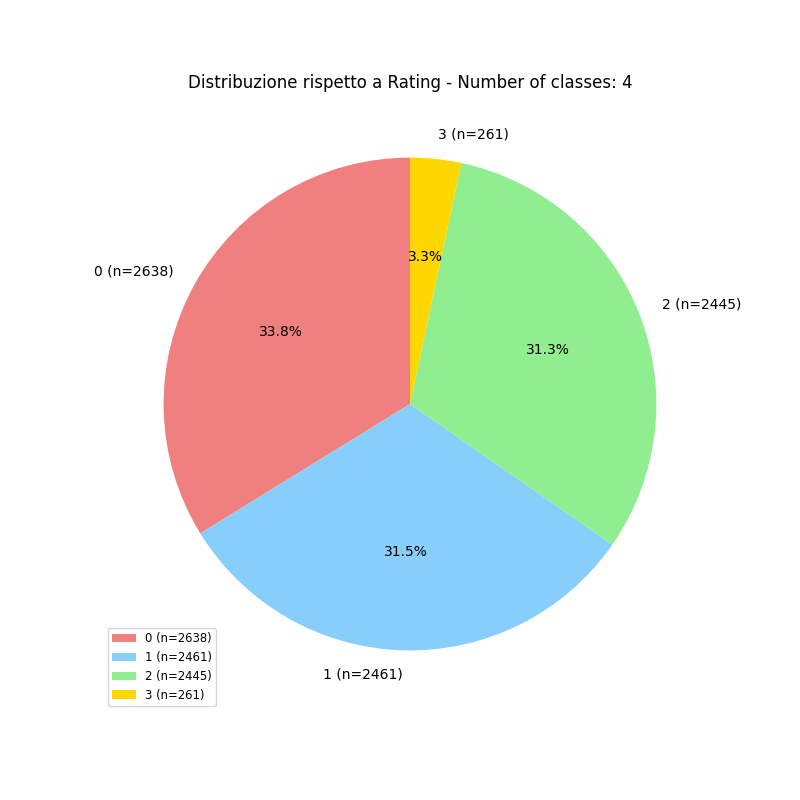
\includegraphics[scale=0.5]{img/class_imbalance.png}
\end{figure}
\noindent Pertanto, quello che stiamo per affrontare è un problema di classificazione multiclasse sbilanciato.